\newcommand{\rendering}[1]{
  \includegraphics[height=\renderingheight]{assets/\clogdirname/pipeline/image_#1.png}
}
\newcommand{\uvmap}[1]{
  \includegraphics[height=\uvheight]{assets/\clogdirname/pipeline/interpolation_#1.png}
}
\newcommand{\modulateduvmap}[1]{
  \includegraphics[height=\renderingheight]{assets/\clogdirname/pipeline/modulated_pred_#1.png}
}
\newcommand{\unmodulateduvmap}[1]{
  \includegraphics[height=\renderingheight]{assets/\clogdirname/pipeline/unmodulated_pred_#1.png}
}
\newcommand{\clogpipelinefig}{
  \def\inputheight{128bp}
  \def\renderingheight{64bp}
  \def\preplasheight{78bp}
  \def\uvheight{52bp}
  \centering
  \font\nullfont=cmr10
  \tikzsetnextfilename{clogpipeline}
  \tikzset{external/export next=false}
  \resizebox{\linewidth}{!}{
    \begin{tikzpicture}[
        >=stealth',
        overlay/.style={
            anchor=south west,
            draw=black,
            rectangle,
            line width=0pt,
            outer sep=0,
            inner sep=0,
          },
      ]
      \node (data) {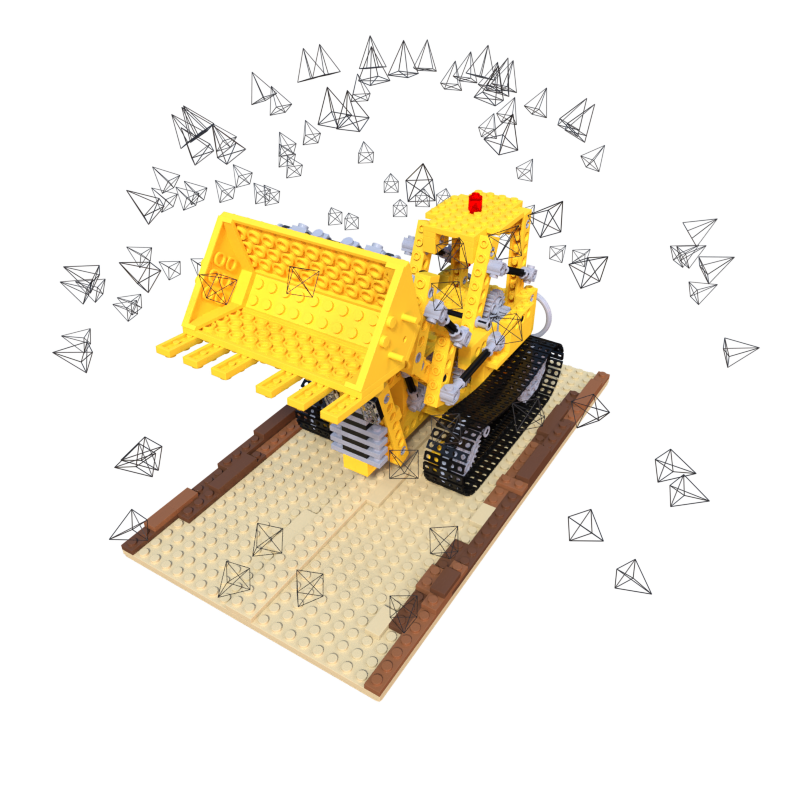
\includegraphics[height=\inputheight]{assets/\clogdirname/pipeline/vis.png}};

      \matrix[
        matrix of nodes,
        right=1em of data,
        column sep=0pt,
        row sep=1.4em,
        ampersand replacement=\&,
        inner sep=0,
        outer sep=0
      ] (pictures) {
        \rendering{0.00} \&
        \rendering{0.25} \&
        \rendering{0.50} \&
        \rendering{0.75} \&
        \rendering{1.00} \\
        \uvmap{0.00} \&
        \uvmap{0.25} \&
        \uvmap{0.50} \&
        \uvmap{0.75} \&
        \uvmap{1.00}     \\
      };
      \node[above right=0em and 0.2em of pictures-2-1.north, scale=0.4] (firstnet) {\rotatebox{90}{\usebox\neuralnet}};
      \node[above=-0.4em of firstnet.north] {\smaller \cref{eq:clog-decoders}};
      \node[above right=0em and 0.2em of pictures-2-2.north, scale=0.4]{\rotatebox{90}{\usebox\neuralnet}};
      \node[above right=0em and 0.2em of pictures-2-3.north, scale=0.4]{\rotatebox{90}{\usebox\neuralnet}};
      \node[above right=0em and 0.2em of pictures-2-4.north, scale=0.4]{\rotatebox{90}{\usebox\neuralnet}};
      \node[above right=0em and 0.2em of pictures-2-5.north, scale=0.4]{\rotatebox{90}{\usebox\neuralnet}};

      \node[right=-1em of data.west, align=center, anchor=base] (stageone) {\rotatebox{90}{Stage I}};
      \node[right=-1.5em of pictures-2-1.west, align=center]{\rotatebox{90}{\smaller Grid of Latents~$\cloglatents$}};
      \node[above=0em of data.north, align=center] {Calibrated cameras};

      \draw[-stealth,  thick, dashed,  ->] ([yshift=4pt]pictures-1-1.north west) -- node [above, midway] {\smaller Training progression and upsampling~(\cref{eq:clog-upsampling})} ([yshift=4pt]pictures-1-5.north east);

      \node[right=1em of pictures.east] (preplas) {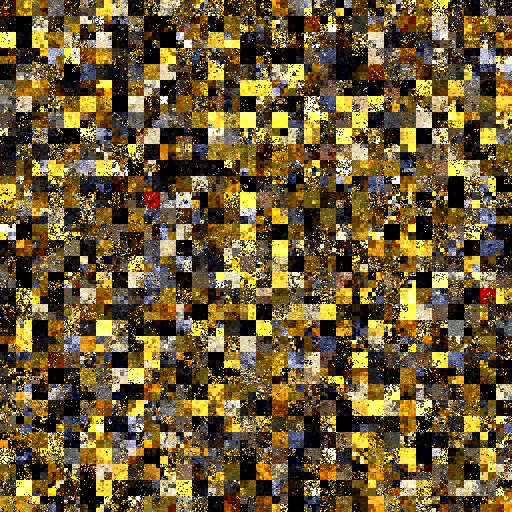
\includegraphics[height=\inputheight]{assets/\clogdirname/plas/unsorted_colors.png}};
      \node[below=3em of preplas.south] (postplas) {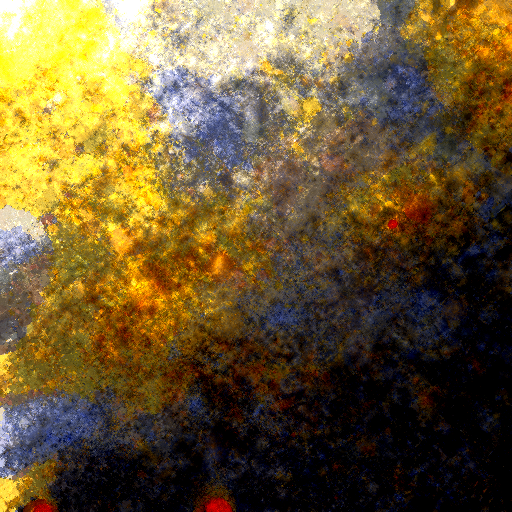
\includegraphics[height=\inputheight]{assets/\clogdirname/plas/sorted_colors.png}};k
      \node[above=0em of preplas.north, align=center] {Trained Grid};

      \draw[-stealth, shorten >= 1pt, shorten <= 1pt,  thick,  ->] (preplas.south) -- node [right, midway] {\smaller PLAS~\cite{morgenstern2024compact}}(postplas.north);

      \node[above left=0.25em and 3.5em of postplas, anchor=north east, scale=1.15] (modulator) {\rotatebox{180}{\usebox\neuralnet}};

      \matrix[
        matrix of nodes,
        left=12em of postplas.west,
        column sep=0pt,
        row sep=0em,
        ampersand replacement=\&,
        inner sep=0,
        outer sep=0
      ] (secondstage) {
        \modulateduvmap{0.00} \&
        \modulateduvmap{0.25} \&
        \modulateduvmap{0.50} \&
        \modulateduvmap{0.75} \&
        \modulateduvmap{1.00}   \\
        \unmodulateduvmap{0.00} \&
        \unmodulateduvmap{0.25} \&
        \unmodulateduvmap{0.50} \&
        \unmodulateduvmap{0.75} \&
        \unmodulateduvmap{1.00} \\
      };
      \draw[-stealth, decoration={snake, pre length=0.01mm, segment length=2mm, amplitude=0.3mm, post length=1.5mm}, decorate, thick] ([yshift=-32bp]postplas.west) -- node [above, midway] {No modulation} (secondstage-2-5);

      \draw[-stealth, decoration={snake, pre length=0.01mm, segment length=2mm, amplitude=0.3mm, post length=1.5mm}, decorate, thick] ([yshift=32bp]postplas.west) -- node [above, midway] {\cref{eq:clog-modulator}} (modulator.east);
      \draw[-stealth, decoration={snake, pre length=0.01mm, segment length=2mm, amplitude=0.3mm, post length=1.5mm}, decorate, thick] (modulator.west) -- node [above, midway] {\cref{eq:clog-modulating}} (secondstage-1-5);

      \node[above=-0.5em of modulator] {Our modulator $\modulator$};

      \node[below=18em of stageone.south, align=center, anchor=base] {\rotatebox{90}{Stage II}};

      \draw[-stealth,  thick, dashed,  ->] ([yshift=0pt]secondstage-1-5.north east) -- node [above, midway] {\smaller Decreasing LoD~$\lod\in[0, 1]$} ([yshift=0pt]secondstage-1-1.north west);

      \node[right=-1.5em of secondstage-1-1.west, align=center] {\small\rotatebox{90}{\textbf{Ours}}};
      \node[right=-1.5em of secondstage-2-1.west, align=center] {\small\rotatebox{90}{For comparison}};

    \end{tikzpicture}
  }
}
\begin{figure}
  \centering
  \clogpipelinefig
  \caption{
    \textbf{Pipeline --}
    We represent the scene with a 2D UV map containing features that an MLP
    interprets 3D Gaussians.
    We first train the UV map at the highest resolution and sort it to ensure
    spatial coherence of similar features, enabling effective subsampling.
    For any desired level of detail (LoD), we obtain the corresponding UV map
    by downsampling and processing it through a modulator that adapts the
    features to map correctly to 3D Gaussians at reduced density.
    This approach enables support for \emph{arbitrary} levels of detail.
  }
  \label{fig:clog-pipeline}
\end{figure}
\section{Related Work}

  We first briefly discuss work on NeRFs~\cite{mildenhall2020nerf} and 3D
  Gaussian Splatting~\cite{kerbl20233d}, then discuss works that focus on
  levels of details.

  \paragraph{Neural Radiance Fields.}
    Neural Radiance Fields (NeRFs)~\cite{mildenhall2020nerf} were introduced
    as a way to incorporate volume rendering within a neural rendering
    pipeline.
    They use a Multi-Layer Perceptron (MLP) to encode the radiance field
    values at each point in the modeling space, which is then volume rendered
    to images.
    Because this volume rendering process is differentiable, given a set of
    images of the same scene with known camera poses, NeRFs can be trained via
    back-propagating through the rendering process for a faithful
    reconstruction of the training images.

    A core limitation of NeRFs is their required compute, which easily took
    multiple days on high-end GPUs for optimal quality.
    Follow-up works thus proposed various ways, using small MLPs divided into
    various regions~\cite{garbin2021fastnerf}, using explicit octree
    representations~\cite{yu2021plenoctrees,fridovich2022plenoxels}, and
    multi-level hashgrids~\cite{mueller2022instant} that eventually allowed
    NeRFs to run in real-time.
    Further enhancements, for example using quantized
    tables~\cite{takikawa2022variable} were also suggested.
    Interestingly, this further allowed NeRF representations to be `streamed'
    at desired resolutions~\cite{reiser2023merf,duckworth2024smerf},
    effectively providing levels-of-detail, similarly to how Neural Geometric
    Level of Detail~\cite{takikawa2021neural} provided LoDs for neural 3D
    shape representations.

  \paragraph{Gaussian Splatting.}
    Even with a hash grid-based implementation~\cite{mueller2022instant}, the
    quality of NeRF renderings highly depends on how points are sampled along
    the light ray.
    On the other hand, 3D Gaussian Splatting (3DGS)~\cite{kerbl20233d} allows
    a deterministic rendering process that does not require this sampling
    process.
    Rather, they represent the radiance values of a 3D scene via 3D Gaussians,
    that are then \emph{rasterized} to images efficiently and differentiably.
    3DGS thus provide super real-time rendering, much faster than the fastest NeRF methods.
    Since the inception of 3DGS, much progress has been made to improve its
    rendering
    quality~\cite{taming3dgs2024mallick,bulo2024revising,huang20242d,jiang2024gaussianshader,liu2024citygaussian,girish2023eagles,kerbl2024hierarchical,radl2024stopthepop,yu2024mip},
    to distill Gaussians into 3D
    voxels~\cite{ren2024octree,lu2024scaffold,liu2024citygaussian} for
    efficient rendering, or to limit the number of Gaussians
    used~\cite{fan2023lightgaussian,niemeyer2024radsplat,lee2024compact,morgenstern2024compact,niedermayr2024compressed,fang2024mini}.
    However, these methods focus on creating a `fixed' compact representation
    for each scene, and always aim for maximum rendering quality---they do not
    have a notion of levels of detail.

  \paragraph{Levels of Detail.}
    Levels of Detail is a well-known technique in computer graphics for
    adapting a target 3D object (usually represented as mesh) to a given
    compute
    budget~\cite{clark1976hierarchical,niessner2012feature,luebke2002level}.
    In the gaming industry, it is commonly used to replace complex 3D objects
    with simpler representations depending on the distance from the player's
    view.
    This method reduces the overall scene complexity without sacrificing its
    fidelity.
    Additionally, they can be used to deliver the object at multiple compute
    budgets.

    In the realm of neural representations, NGLOD~\cite{takikawa2021neural}
    proposed to produce a signed distance field in a continuous matter.
    In a similar spirit, Variable Bitrate Neural
    Fields~\cite{takikawa2022variable} quantize the latent vectors of the
    radiance field to enable field streaming.
    These methods, however, are not trivial to extend to 3DGS, which optimizes
    each of the Gaussians independently and uses non-differentiable heuristics
    to minimize the reconstruction error.

    Octree-GS~\cite{ren2024octree} introduced levels of detail with Gaussian
    splatting by learning an adaptive partition of 3D space (an octree) that
    naturally induces a hierarchy of details into the scene.
    The method is closely related to Scaffold-GS~\cite{lu2024scaffold}, as
    they both start from points obtained from
    Structure-from-Motion~\cite{schonberger2016structure} for their
    representation, but expands their view-dependent rendering to select
    anchors and Gaussian parameter offsets from multiple LODs during
    inference.
    A recent method, FLoD~\cite{seo2024flod}, introduces a less structured
    approach that simply trains using multiple stages, where each stage is
    dedicated to a `level' of detail, and optionally selects a subset of
    levels at runtime.
    During training, FLoD constrains the scale of the Gaussians at each level,
    effectively using large Gaussians for coarser levels, later learning
    fine-grained details with smaller Gaussians.
    While these strategies do allow for levels of detail with 3DGS, they only
    do so at fixed pre-defined intervals, limiting their applicability.

    In our work, we draw inspiration from Mixed Volumetric Primitives
    (MVP)~\cite{raj2021pixel,lombardi2021mixture} and Relightable Gaussian
    Codec Avatars (RGCA)~\cite{saito2024relightable} and approach the problem
    of 3D reconstruction from the perspective of a deterministic,
    pixel-aligned 2D to 3D mapping.
    Our key idea is that once this 2D-to-3D mapping is learned, we can
    subsample the 2D image to create a continuous LoD.
    Using 2D images was also explored in TextureGS~\cite{xu2024texturegs},
    where this idea was used to disentangle texture from appearance.
    Here, we show that this 2D image can do much more---it can be used to
    group Gaussians together, creating a representation that can be used to
    provide continuous levels of detail for 3D Gaussian Splatting.

